\chapter{Discussion on Results}

By examining the network problem data,
we can see that the number of OD pairs increase
significantly respect to the number of zone nodes,
this is important because it indicates how many point to point SPPs need to be solved for each iteration of the PE method.
We can also roughly tell that these networks are very sparse;
for a complete graph (every node is connected to every other node) of 1000 nodes have 499500 edges ($n(n-1)/2$),
but the larger networks in our problem data only have about 0.4\% to 0.6\% of edges in the corresponding complete graph. 
Analysing the graph shows the degree of any vertex in the graph is no more than 5.
This information is useful for choosing the best algorithm and data structure.

Now we investigate the reason for the run time behaviours of the shortest path algorithms shown in Figure~\ref{fig:allresults}.
Figure~\ref{fig:long_sptree} shows the shortest path trees of the point-to-point algorithms, where the origin and destination node is placed on the opposite side of the ChicagoSketch network.
It can be seen that Dijkstra's algorithm scans the entire network;
the Bidirectional Dijkstra scans almost the whole network but with a few nodes left out;
The Bidirectional A* search scans a slightly larger region near the origin and destination nodes;
and the A* search only scans a few nodes along the shortest path.
The behaviour of the algorithms is shown further in Figure~\ref{fig:short_sptree},
where the origin and destination is placed close to each other.
The Dijkstra and Bidirectional Dijkstra algorithm need to scan many nodes before termination;
And the A* and Bidirectional A* search only scan a small portion of network,
and they do not scan the area behind the origin and destination node.

The run time of the shortest path algorithms are heavily dependent on the number of nodes they scan.
The process of scanning a node consists of placing the node into a priority queue, taking it out sometime later, and check all its out going arcs.
So cumulatively the less nodes an algorithm scans the faster it runs.
And by examining Figure~\ref{fig:long_sptree} and Figure~\ref{fig:short_sptree},
it is obvious to see A* search is the fastest.

\begin{figure}
    \centering
    \begin{subfigure}{.5\textwidth}
        \centering
        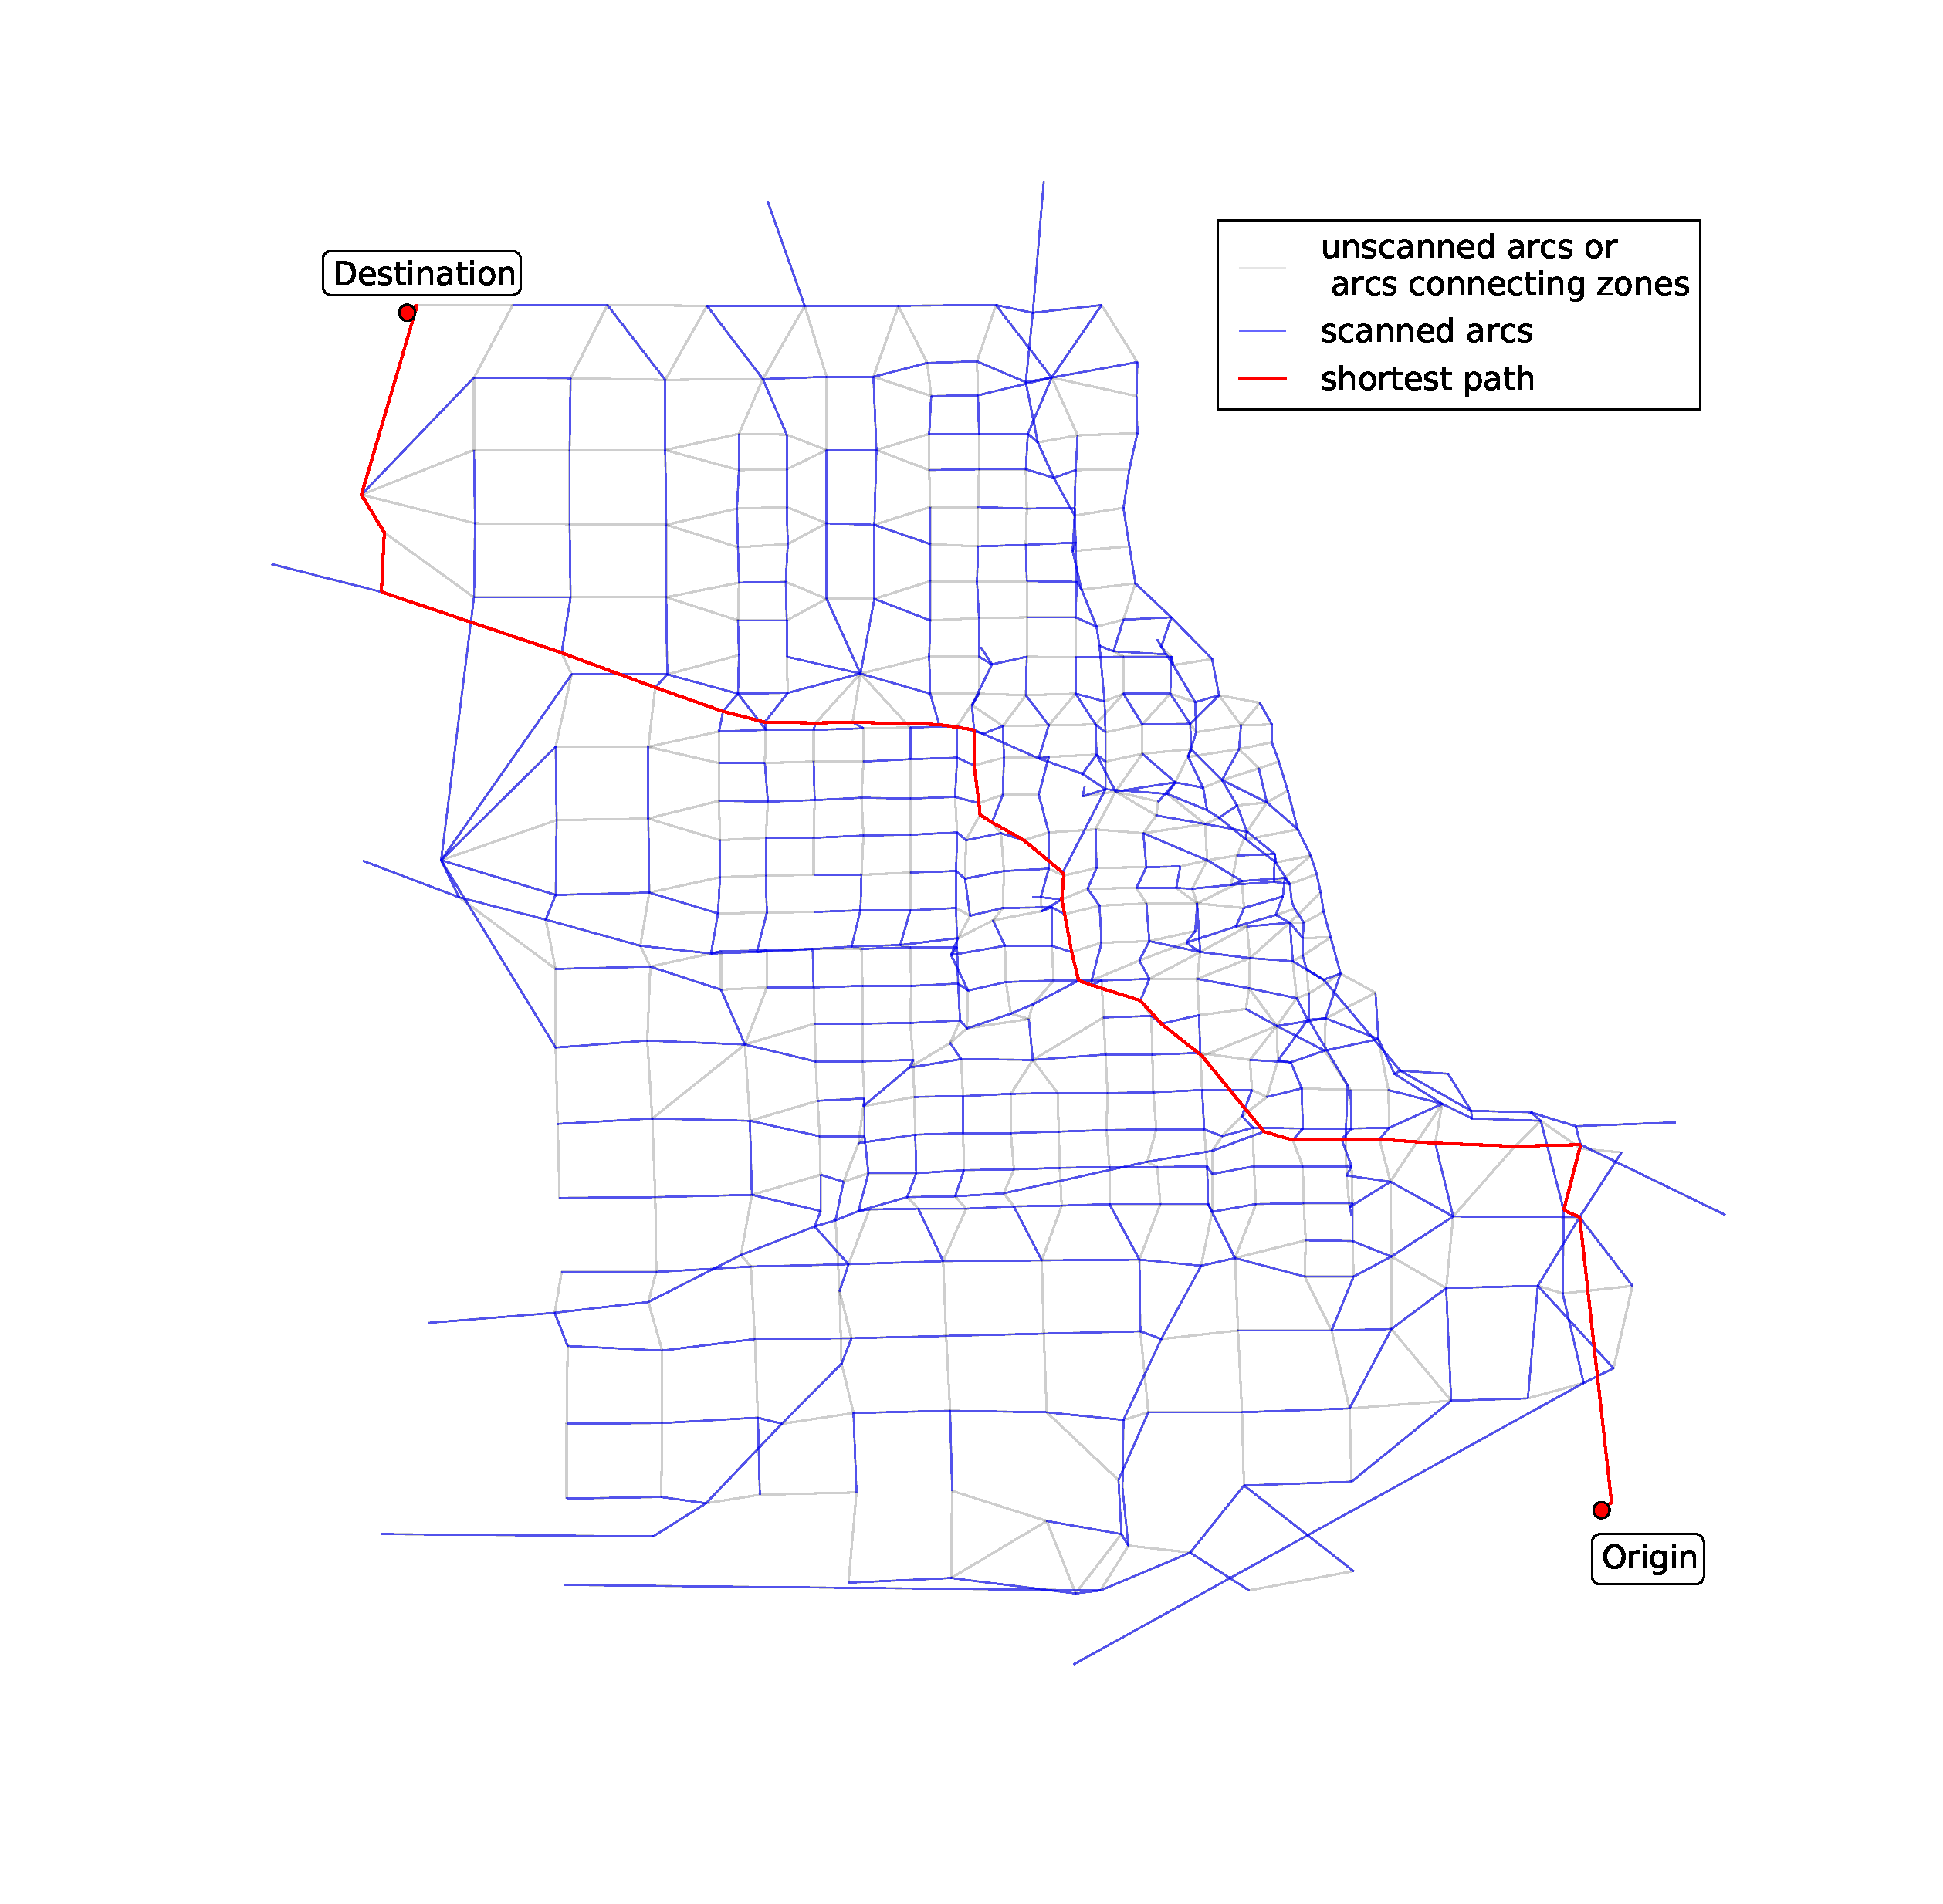
\includegraphics[width=\textwidth,trim=120px 120px 48px 120px,clip]{img/chicago_dijkstra}
        \caption{Dijkstra}
        \label{fig:chicago_dijkstra}
    \end{subfigure}%
    \begin{subfigure}{.5\textwidth}
        \centering
        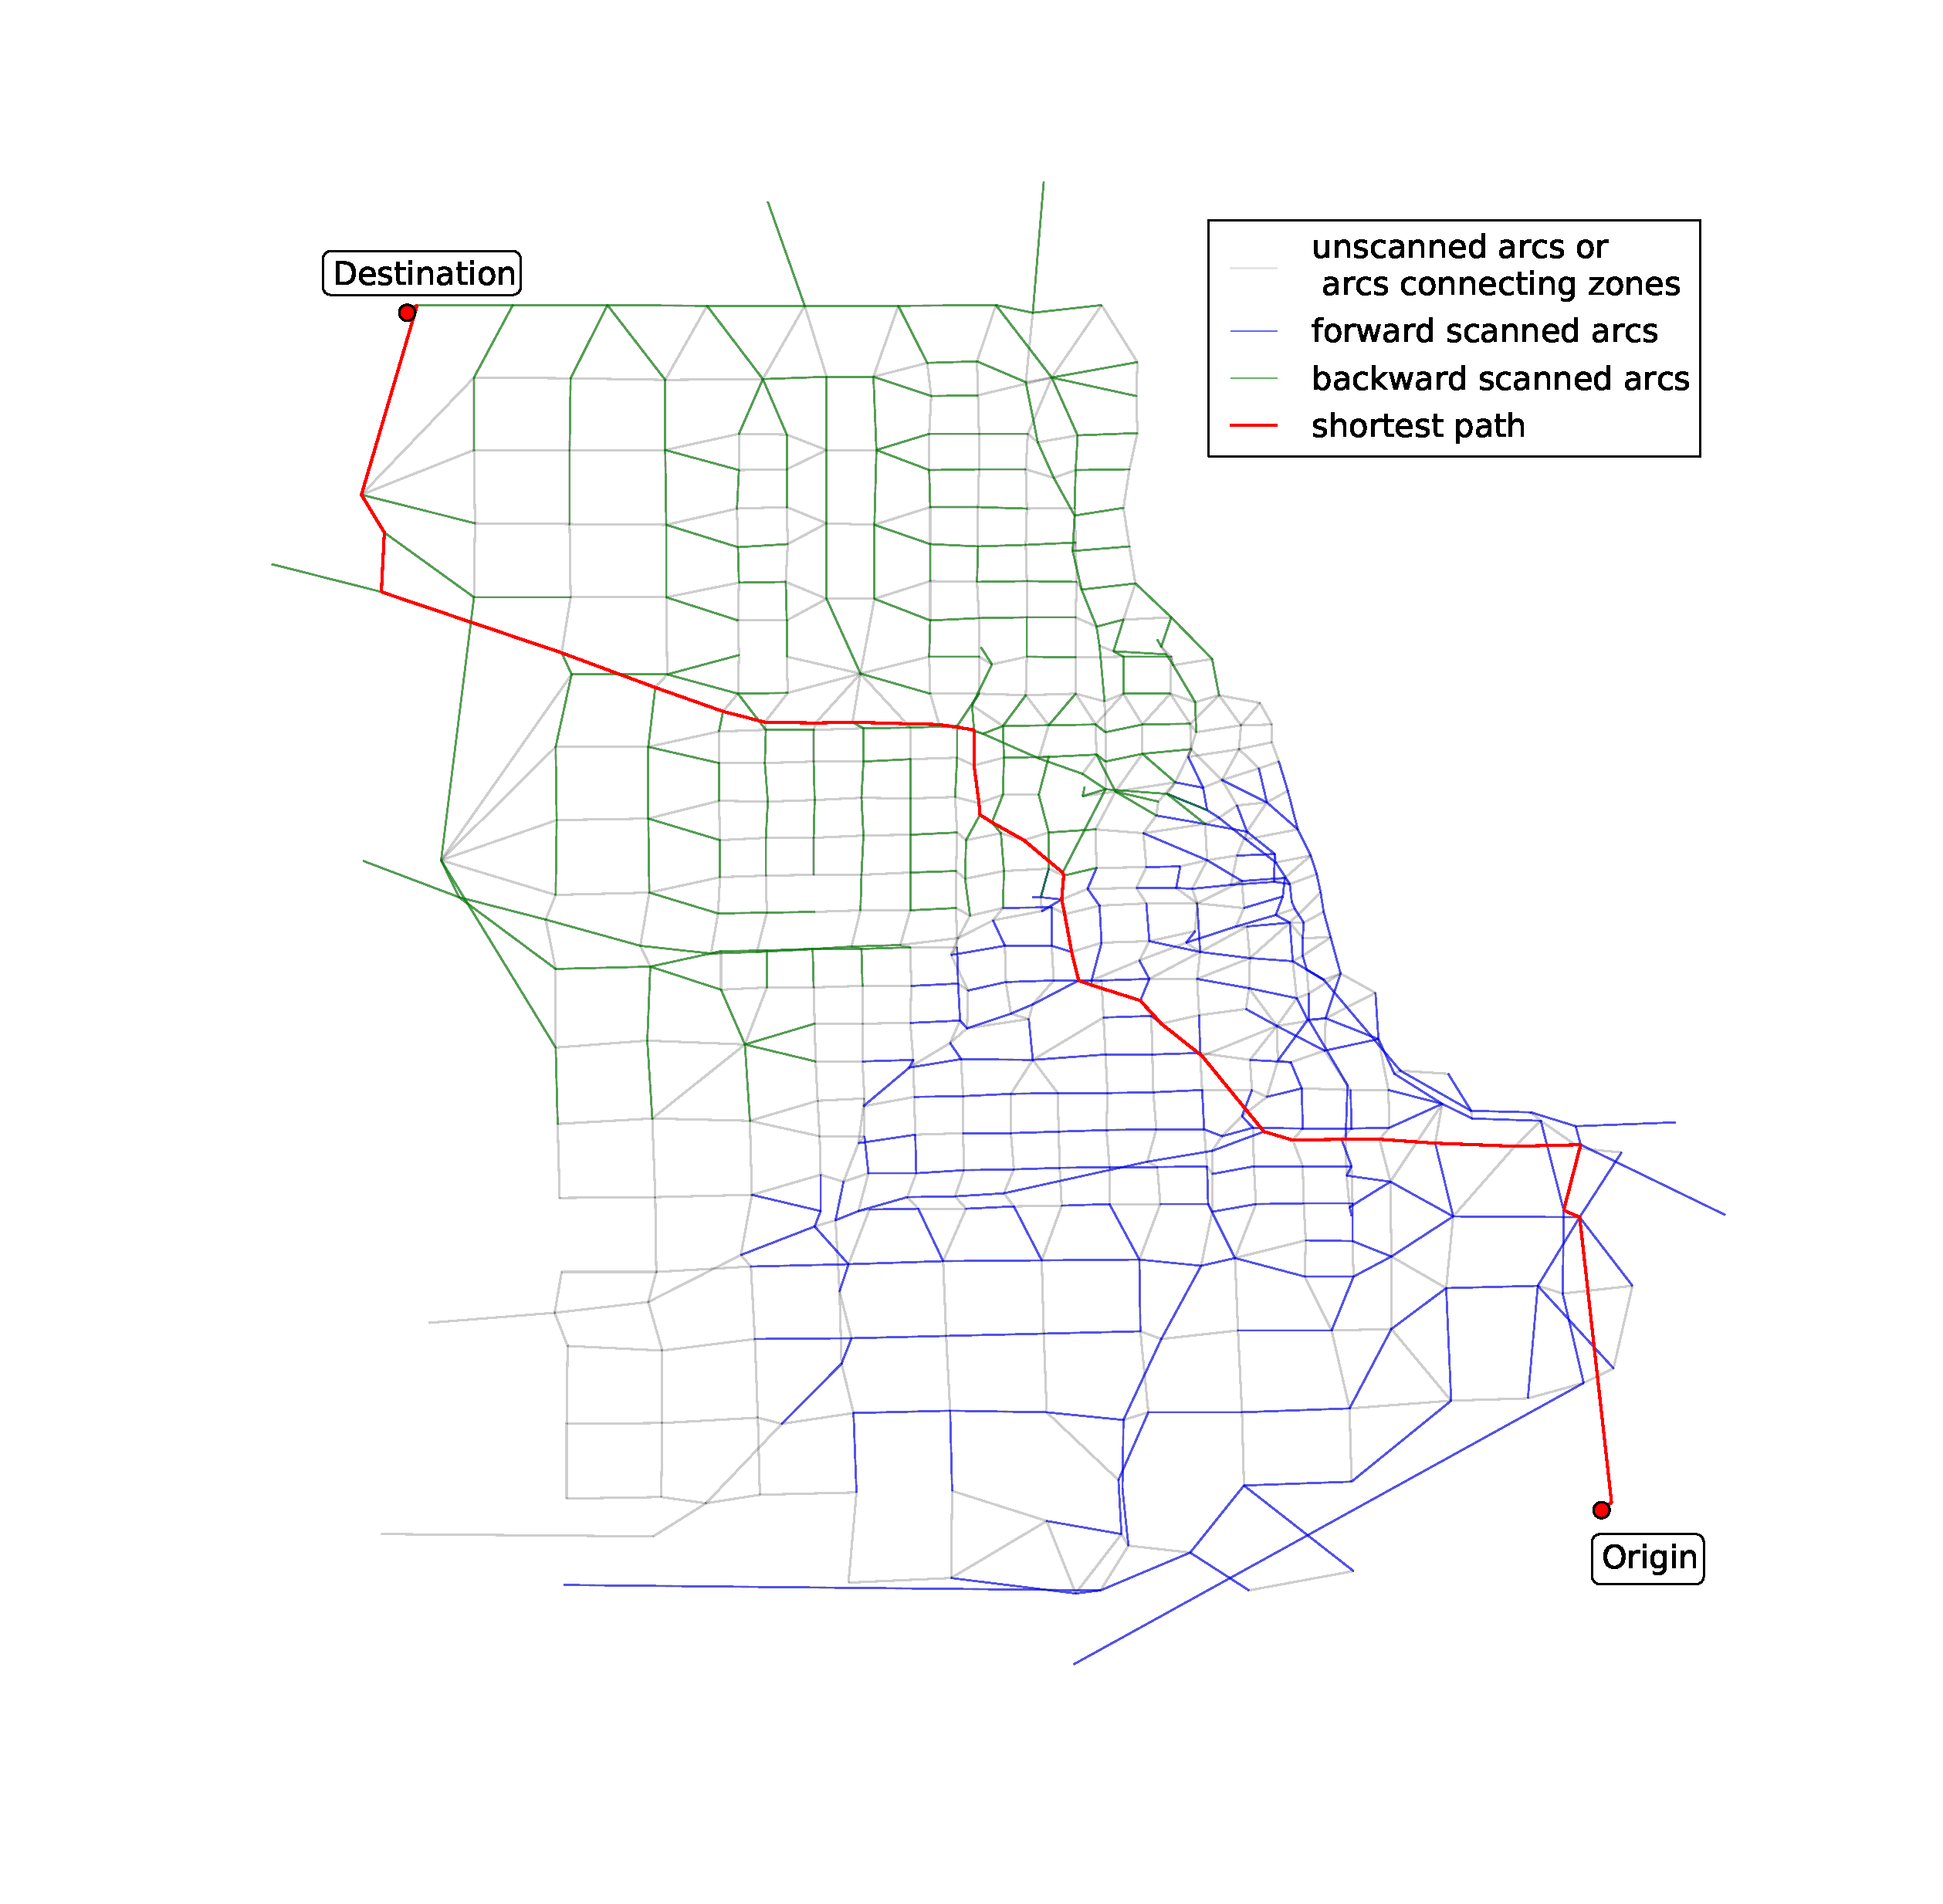
\includegraphics[width=\textwidth,trim=120px 120px 48px 120px,clip]{img/chicago_bidirect}
        \caption{Bidirectional Dijkstra}
        \label{fig:chicago_bidirect}
    \end{subfigure}
    \begin{subfigure}{.5\textwidth}
        \centering
        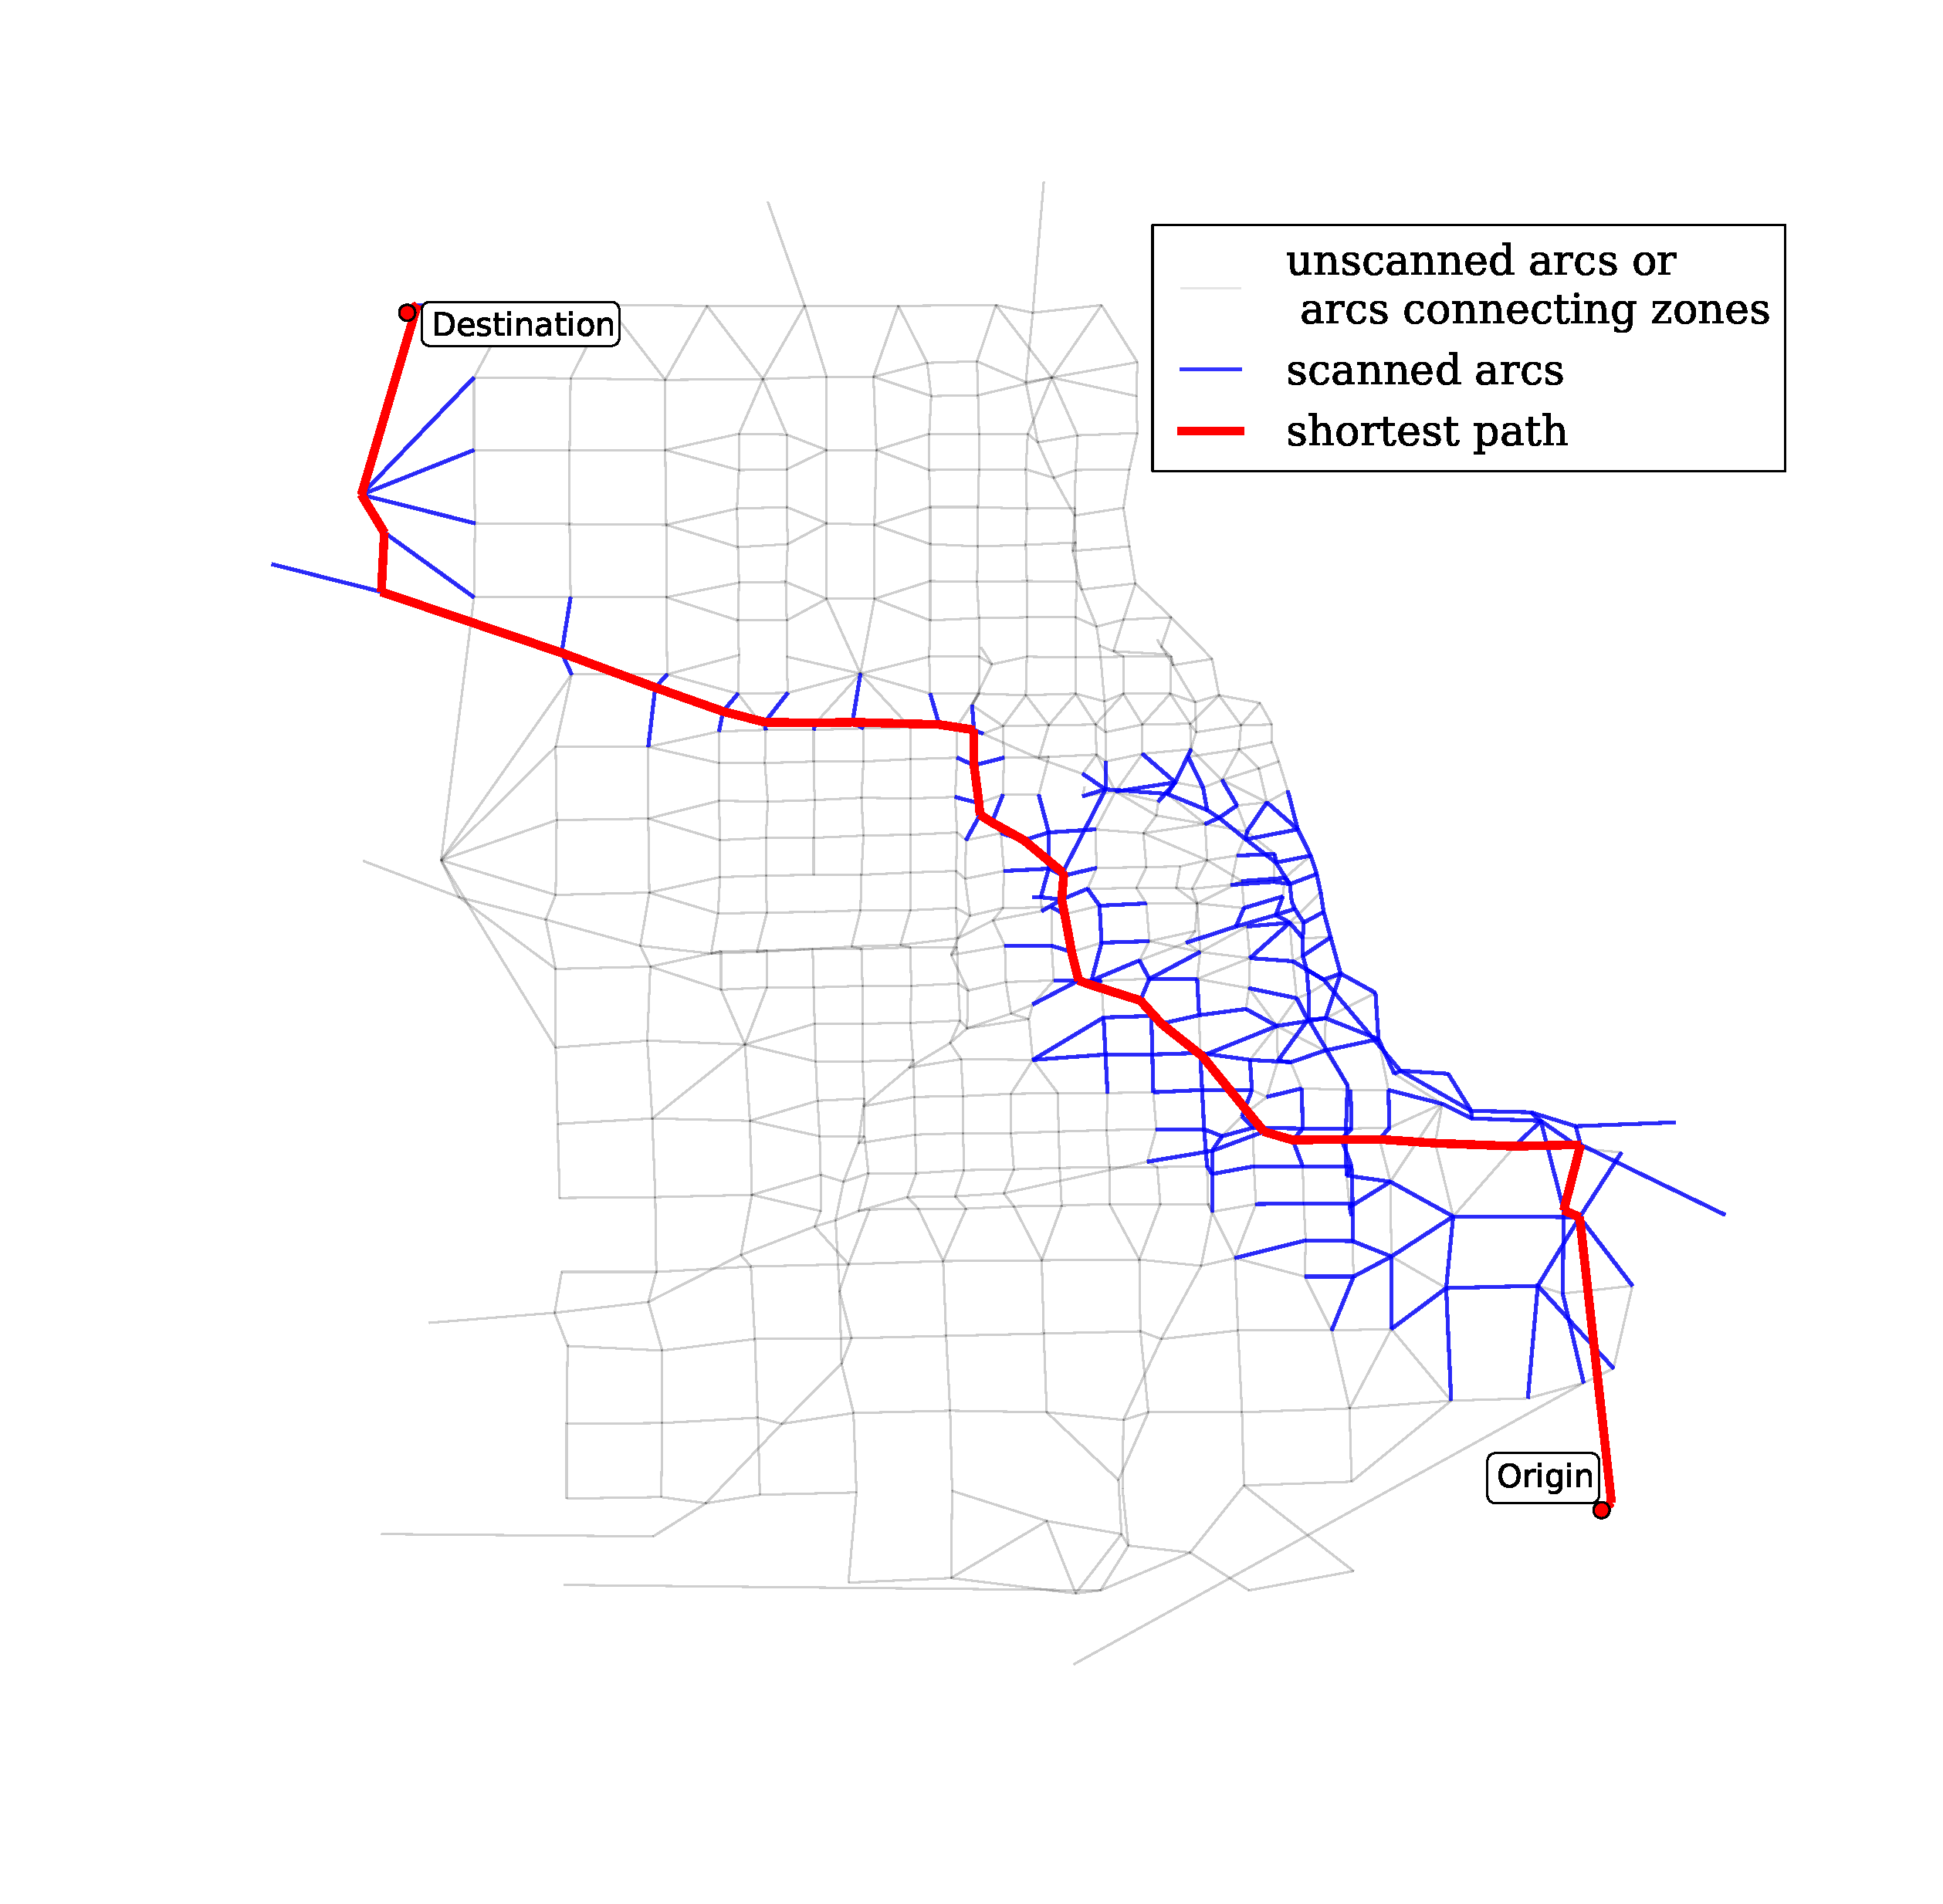
\includegraphics[width=\textwidth,trim=120px 120px 48px 0px,clip]{img/chicago_astar}
        \caption{A* Search}
        \label{fig:chicago_astar}
    \end{subfigure}%
    \begin{subfigure}{.5\textwidth}
        \centering
        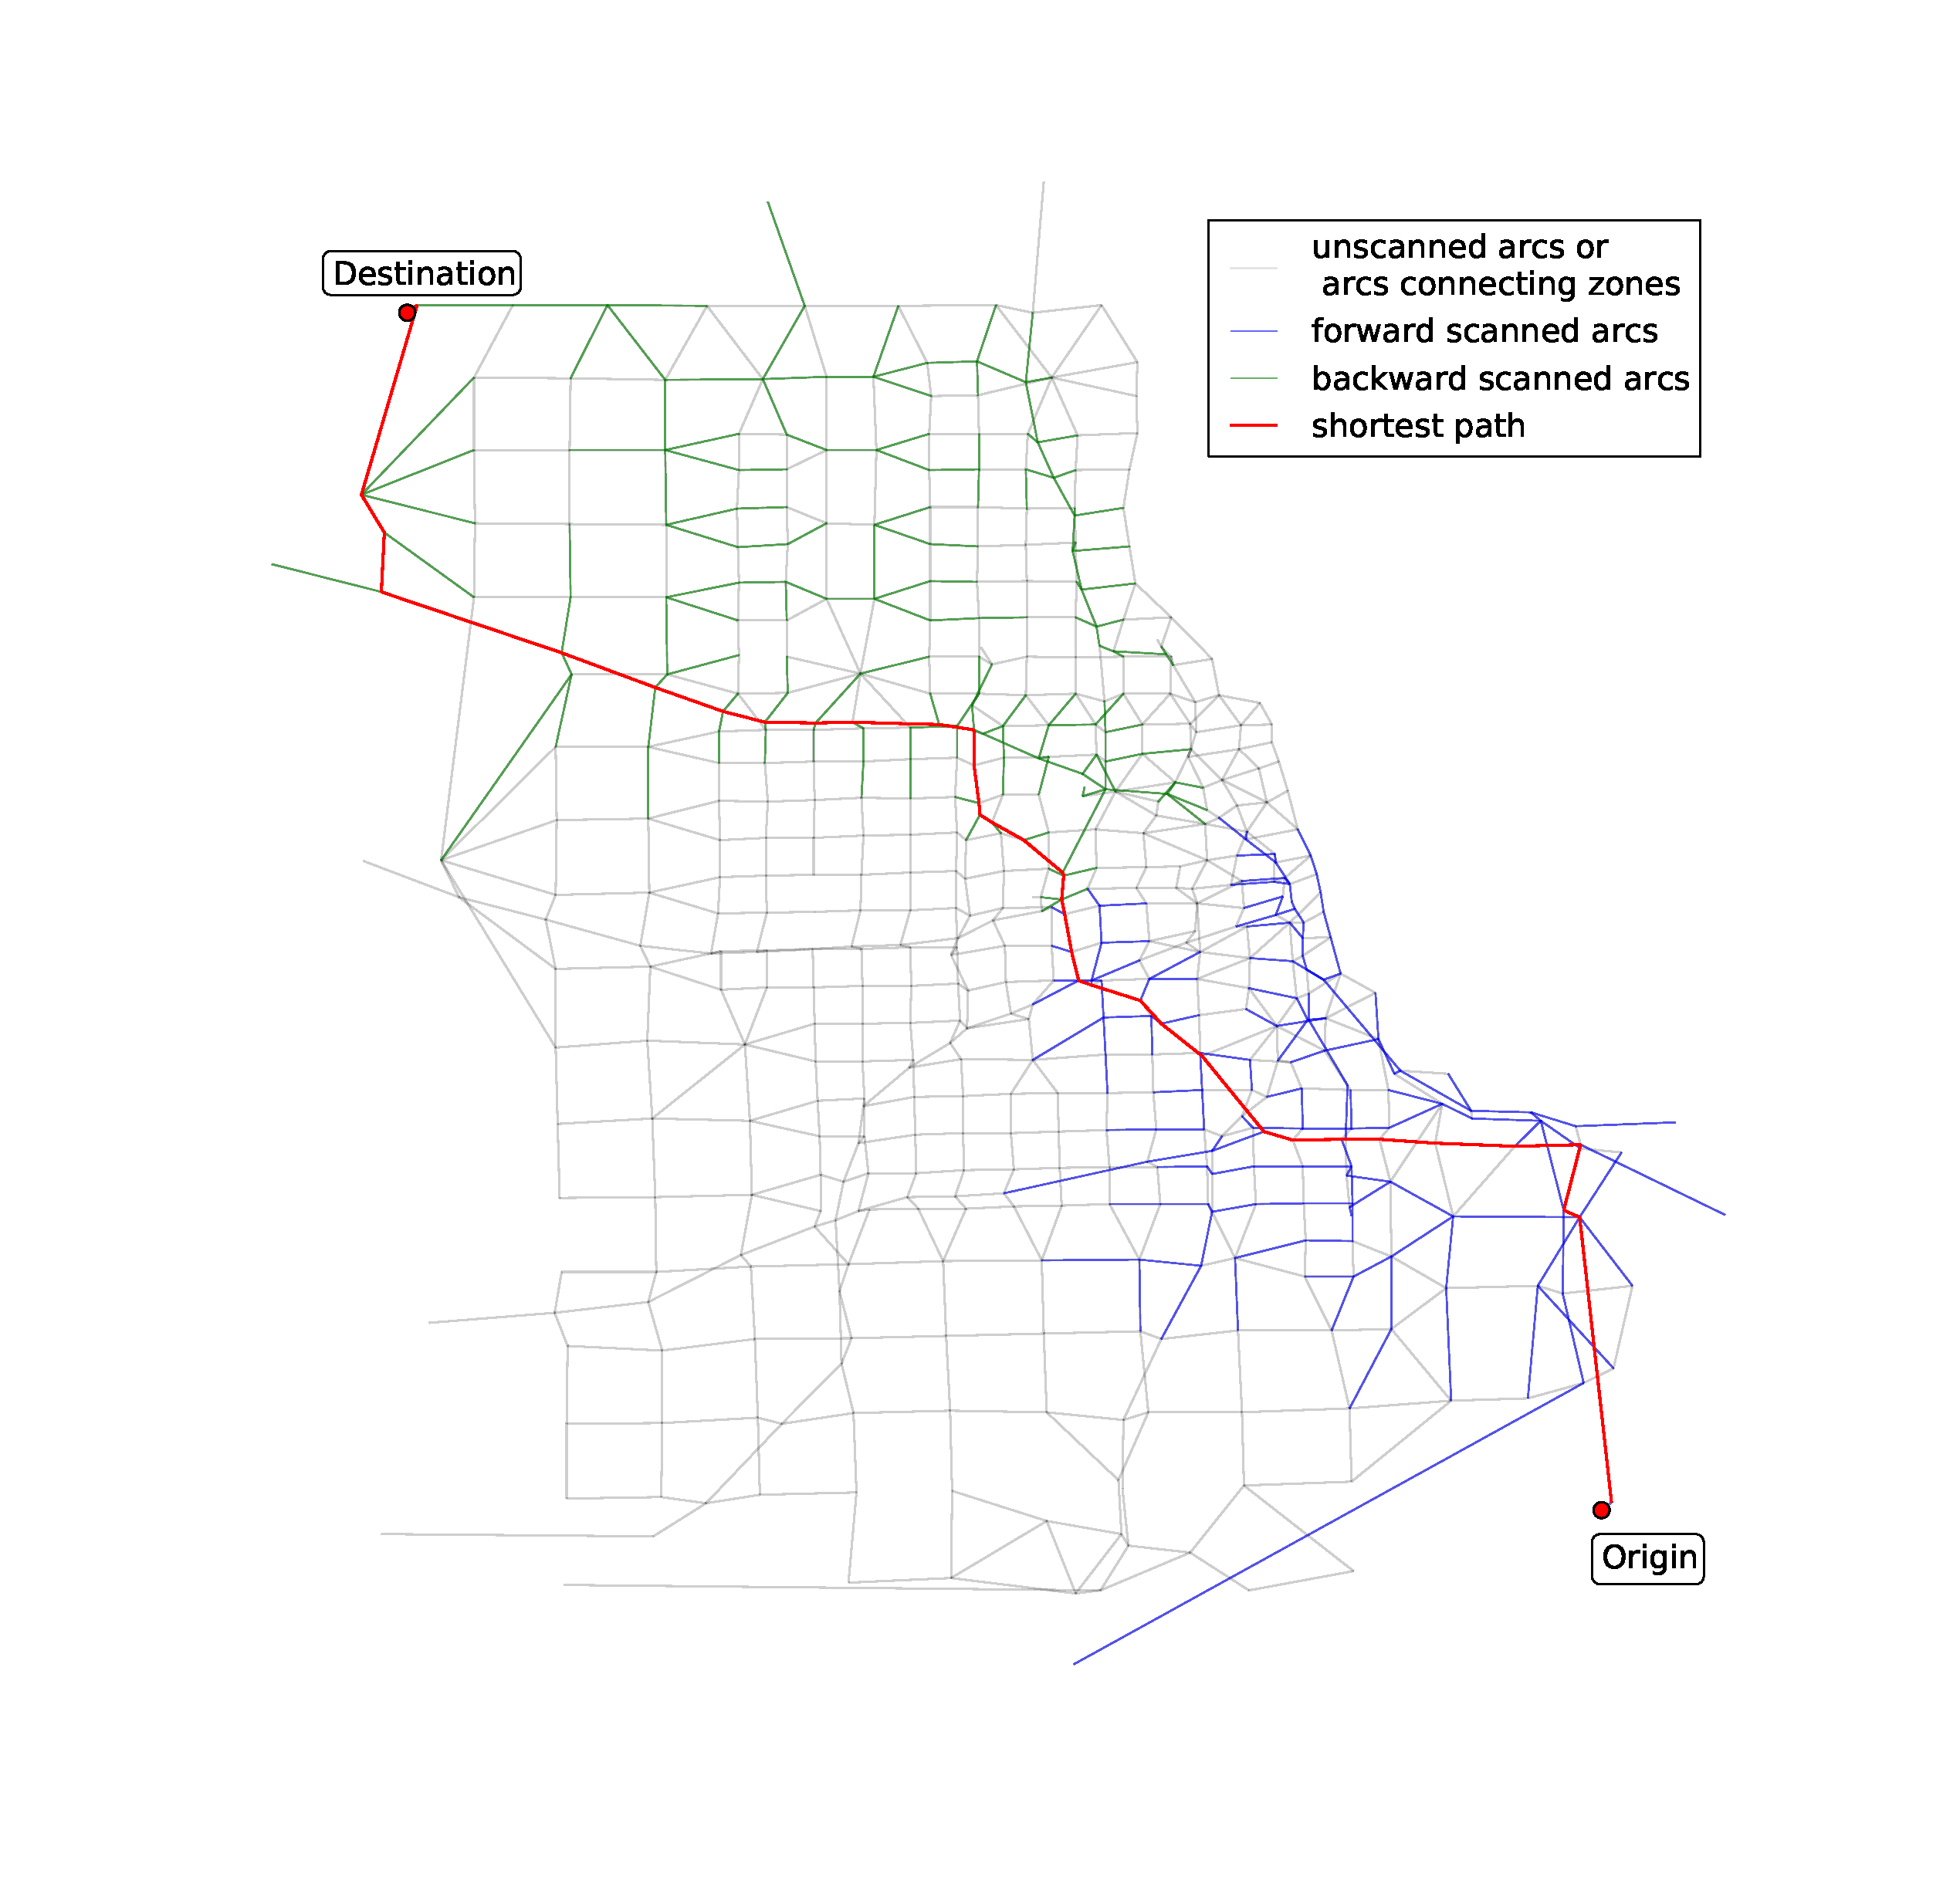
\includegraphics[width=\textwidth,trim=120px 120px 48px 0px,clip]{img/chicago_astar_bidirect}
        \caption{Bidirectional A* Search}
        \label{fig:chicago_astar_bidirect}
    \end{subfigure}
    \vspace{1em}
    \caption{Shortest path tree between two distant nodes in the ChicagoSketch Network}
    \label{fig:long_sptree}
\end{figure}

\begin{figure}
    \centering
    \begin{subfigure}{.5\textwidth}
        \centering
        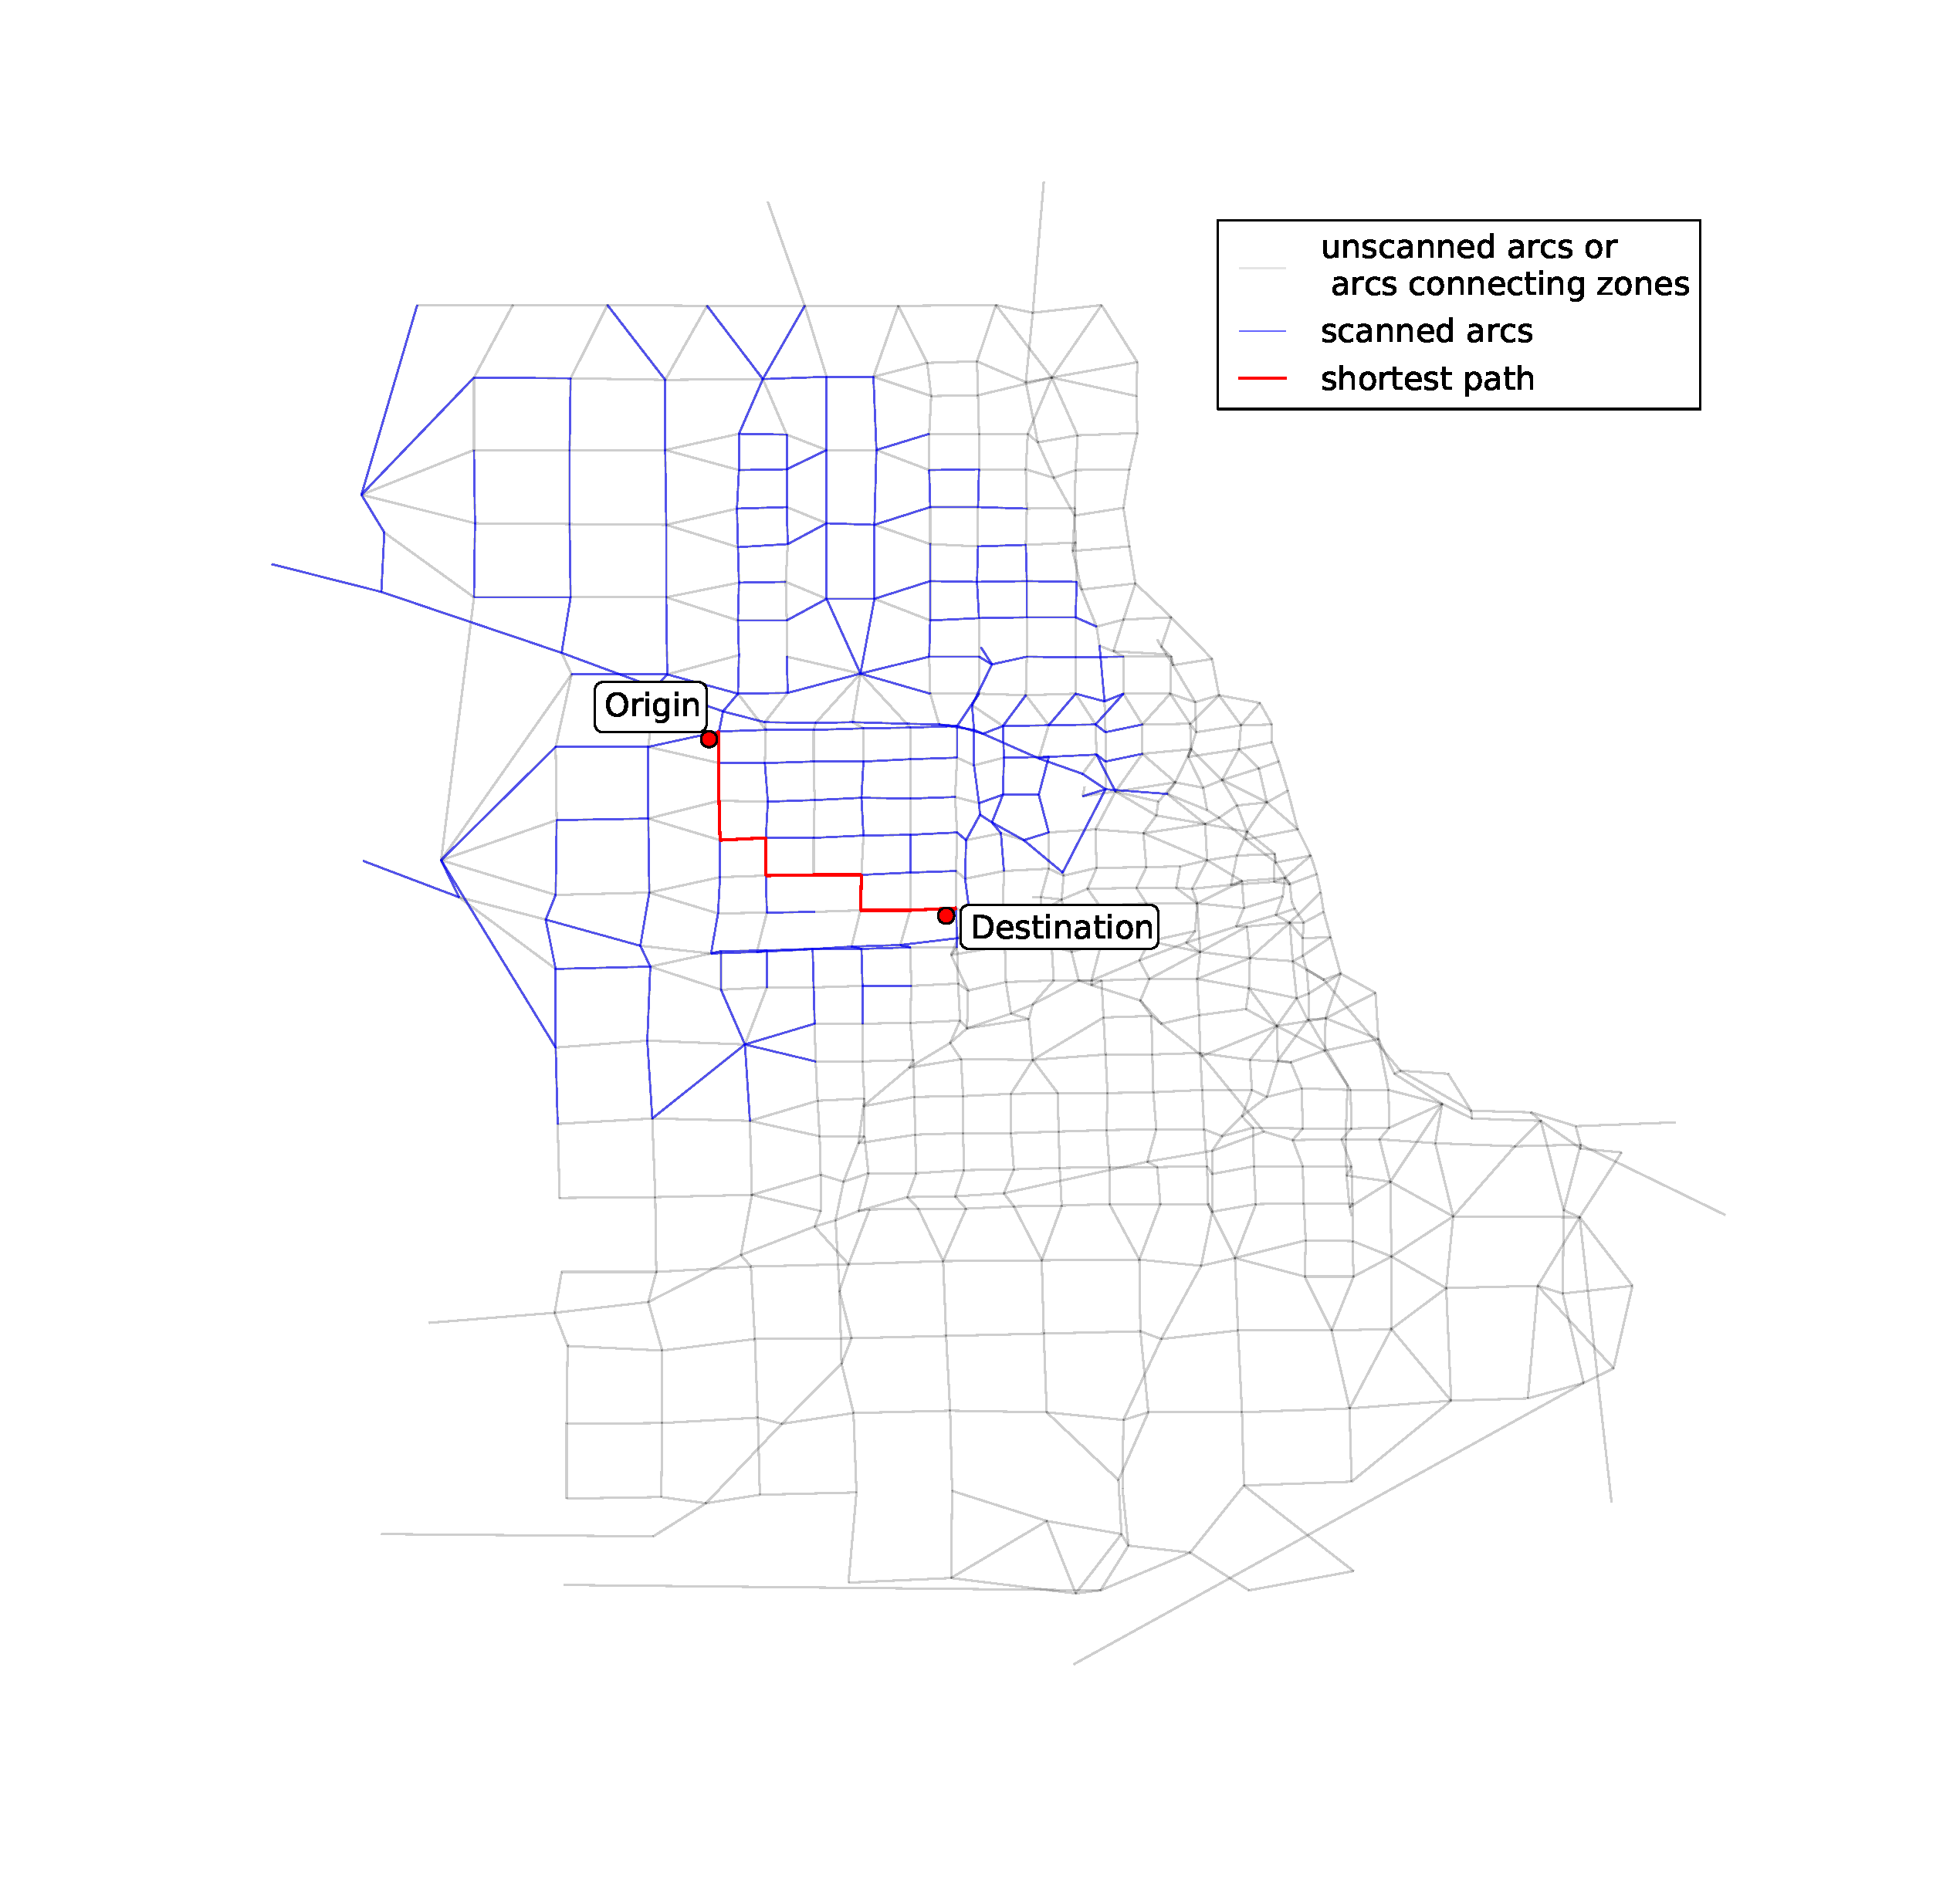
\includegraphics[width=\textwidth,trim=120px 120px 48px 120px,clip]{img/chicago_dijkstra2}
        \caption{Dijkstra}
        \label{fig:chicago_dijkstra2}
    \end{subfigure}%
    \begin{subfigure}{.5\textwidth}
        \centering
        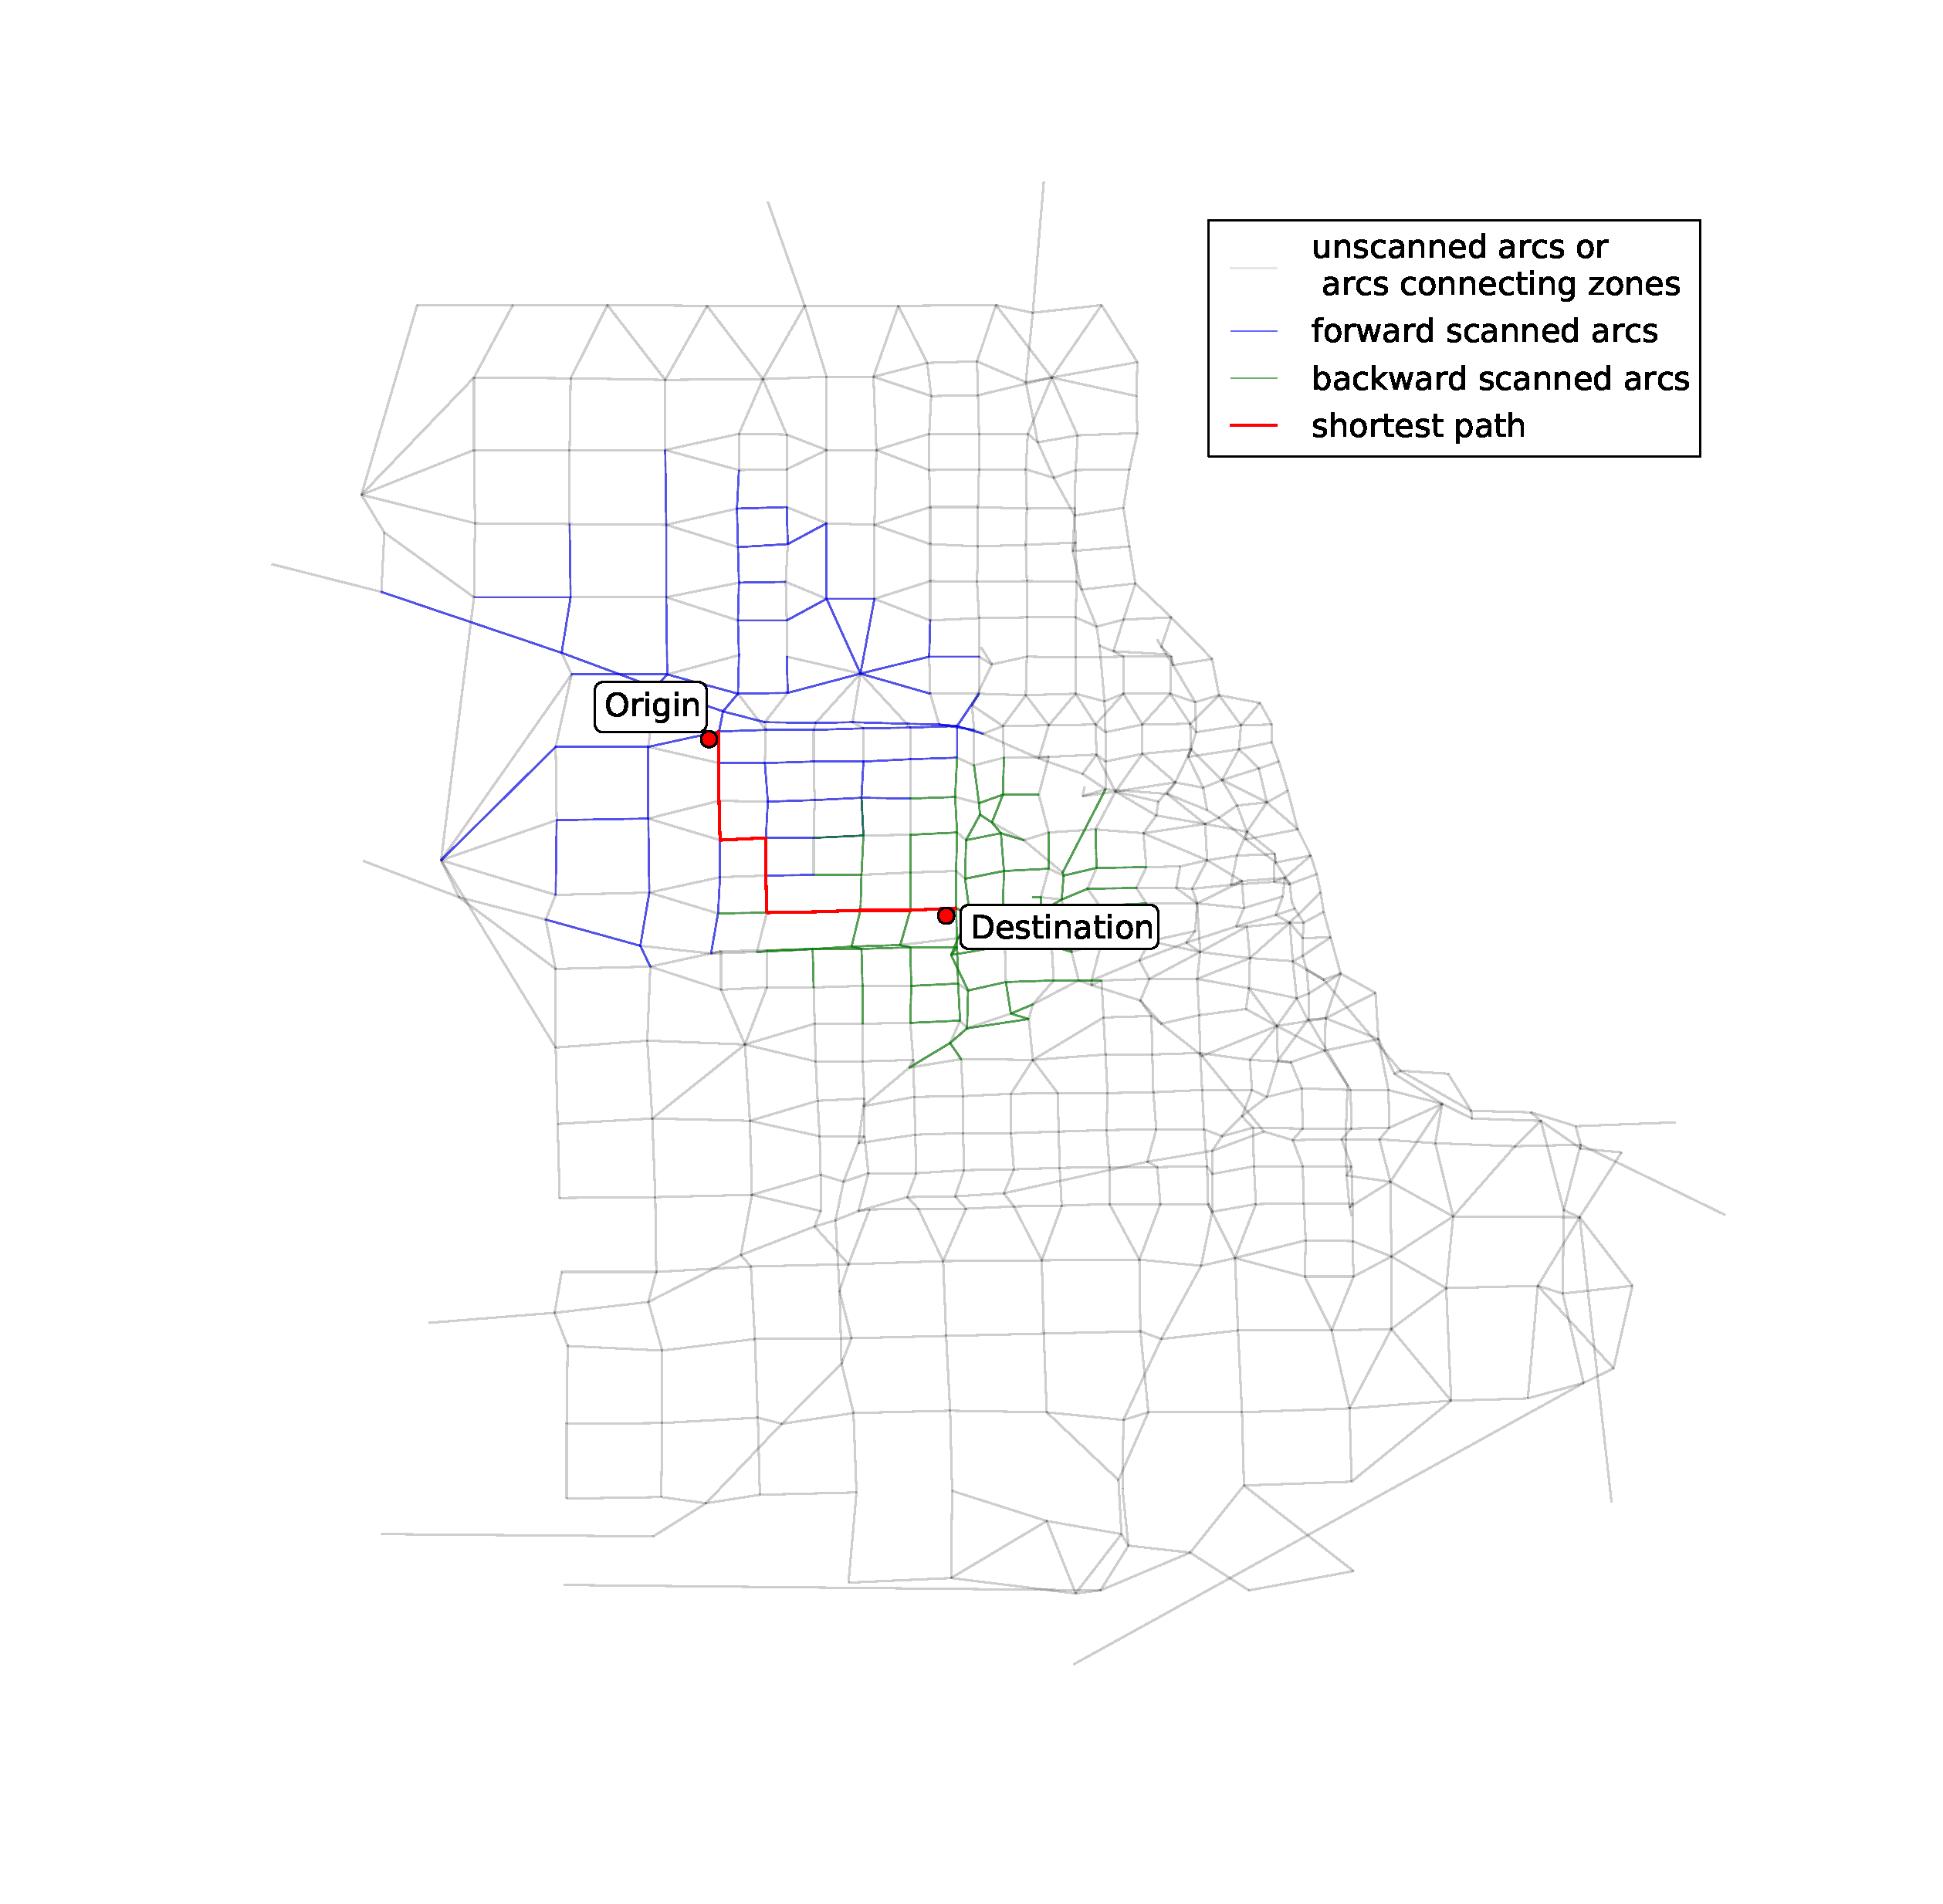
\includegraphics[width=\textwidth,trim=120px 120px 48px 120px,clip]{img/chicago_bidirect2}
        \caption{Bidirectional Dijkstra}
        \label{fig:chicago_bidirect2}
    \end{subfigure}
    \begin{subfigure}{.5\textwidth}
        \centering
        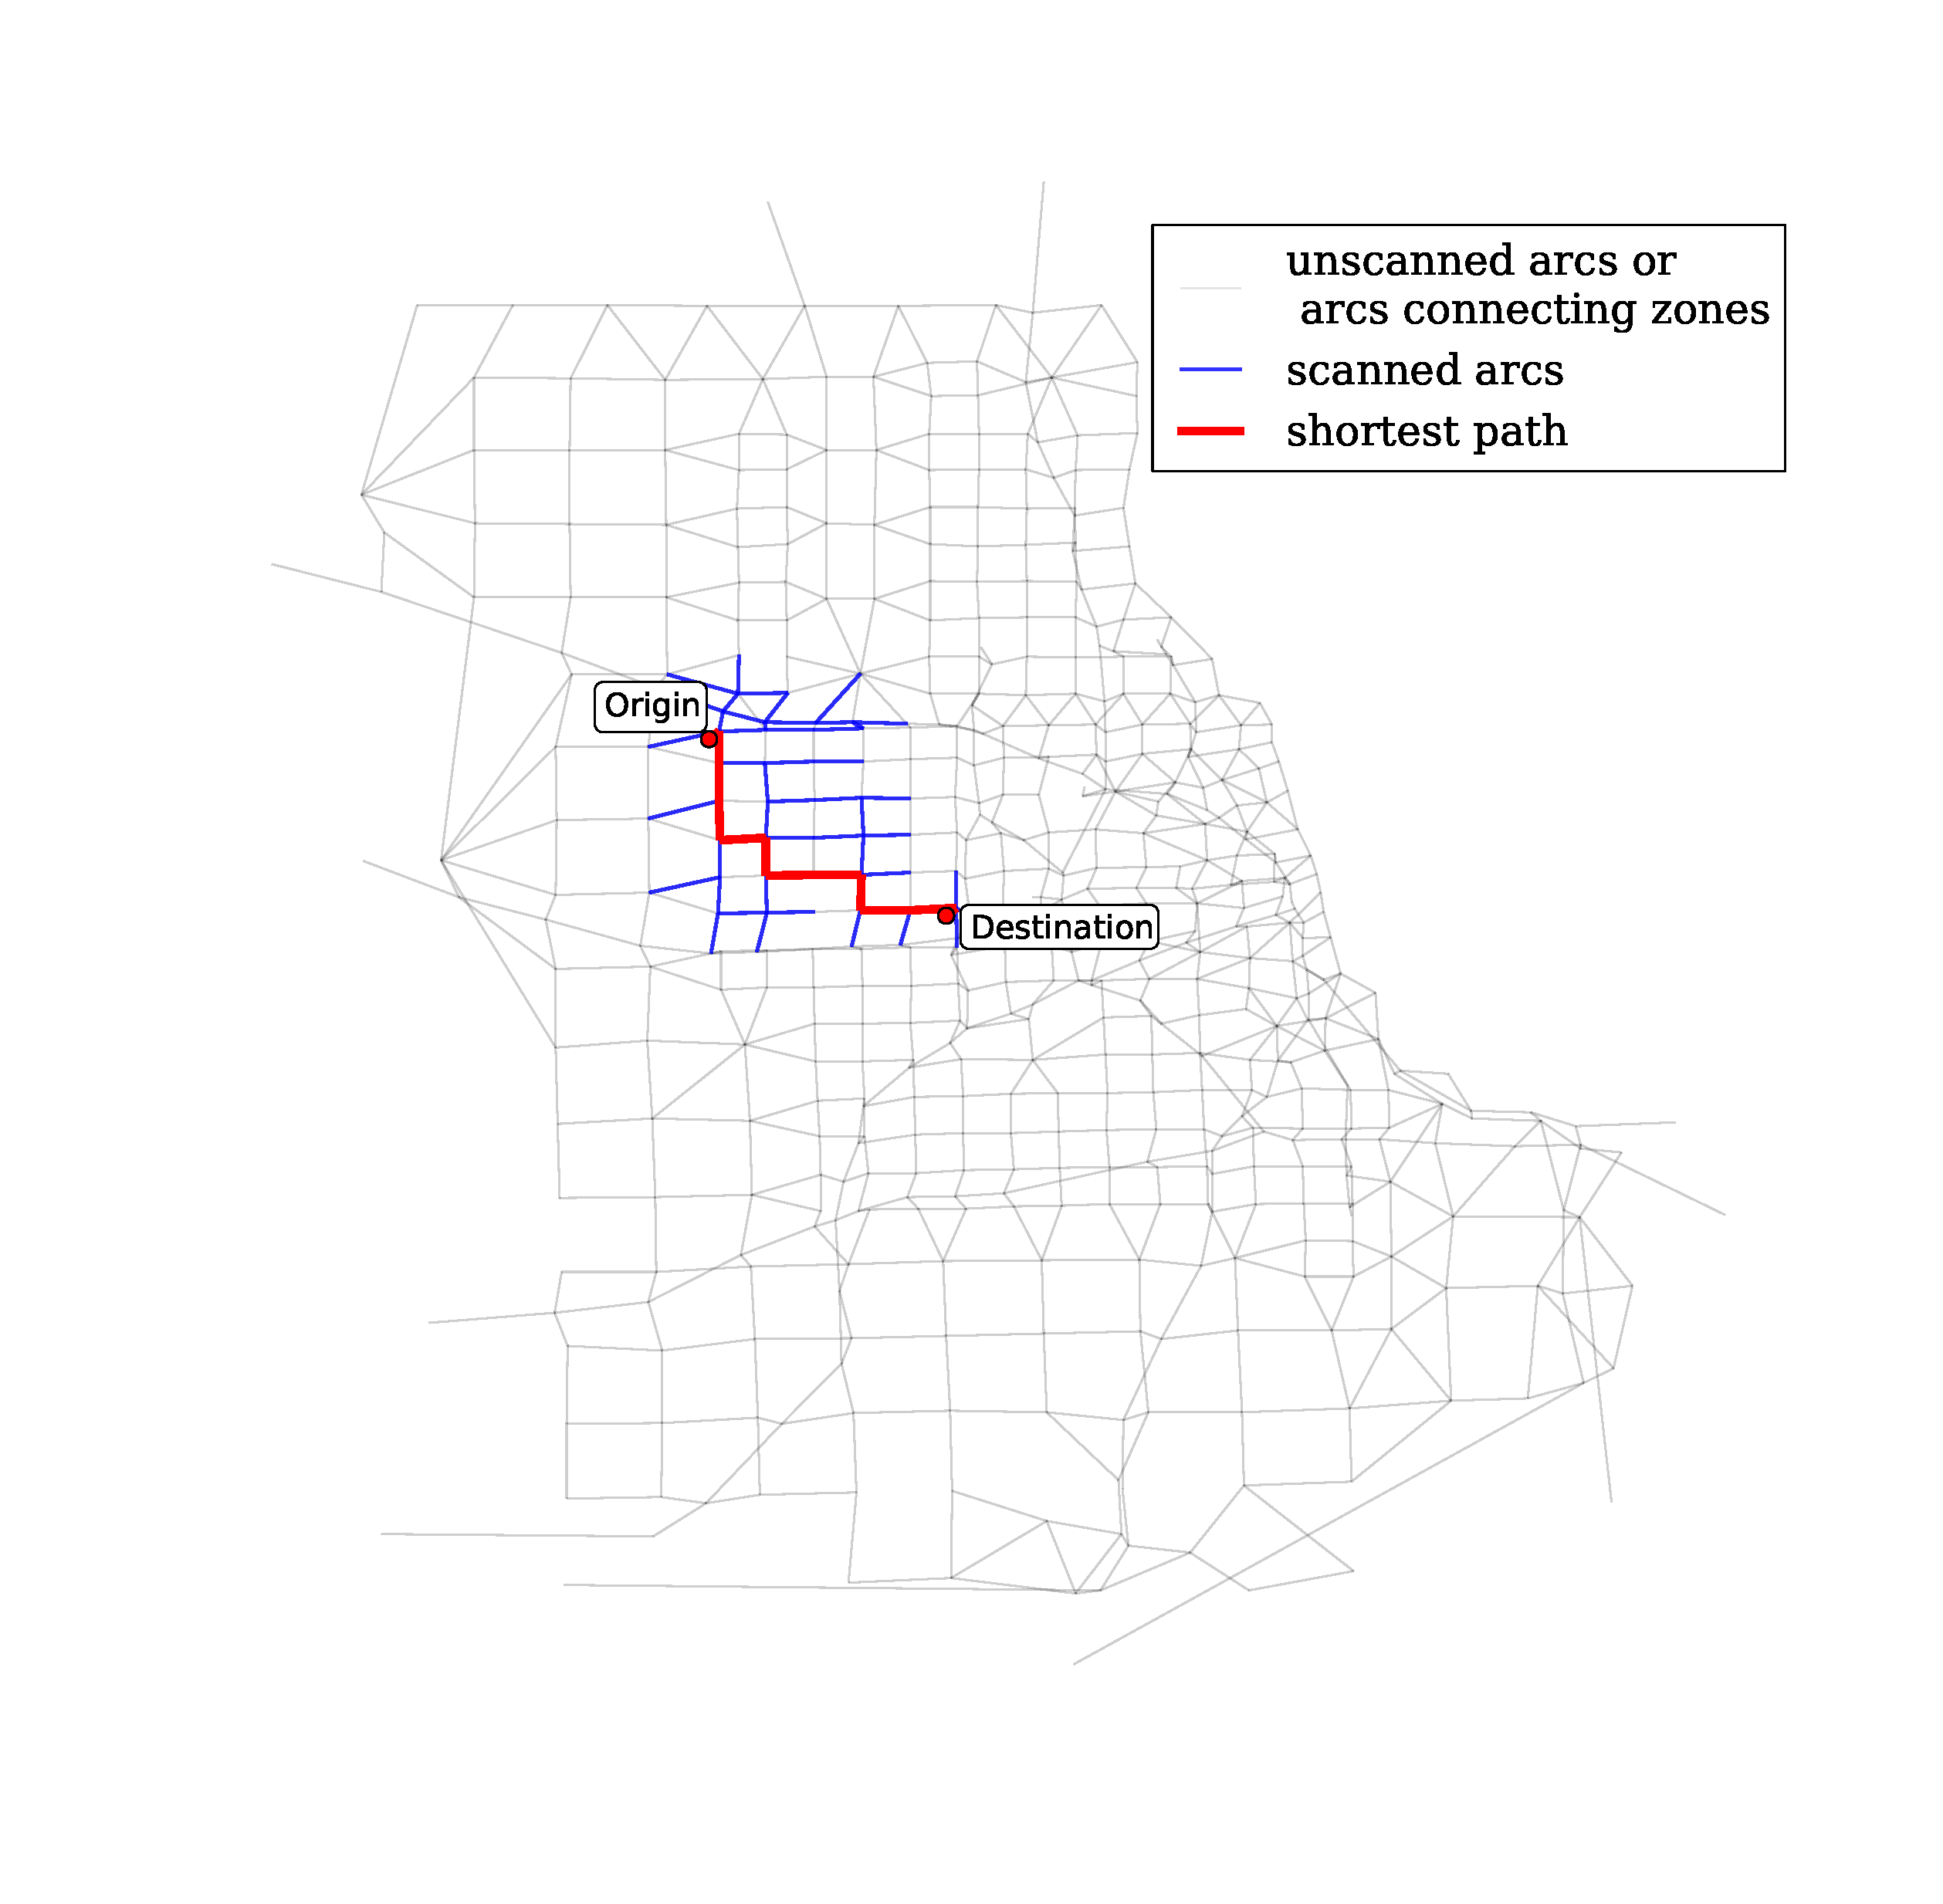
\includegraphics[width=\textwidth,trim=120px 120px 48px 0px,clip]{img/chicago_astar2}
        \caption{A* Search}
        \label{fig:chicago_astar2}
    \end{subfigure}%
    \begin{subfigure}{.5\textwidth}
        \centering
        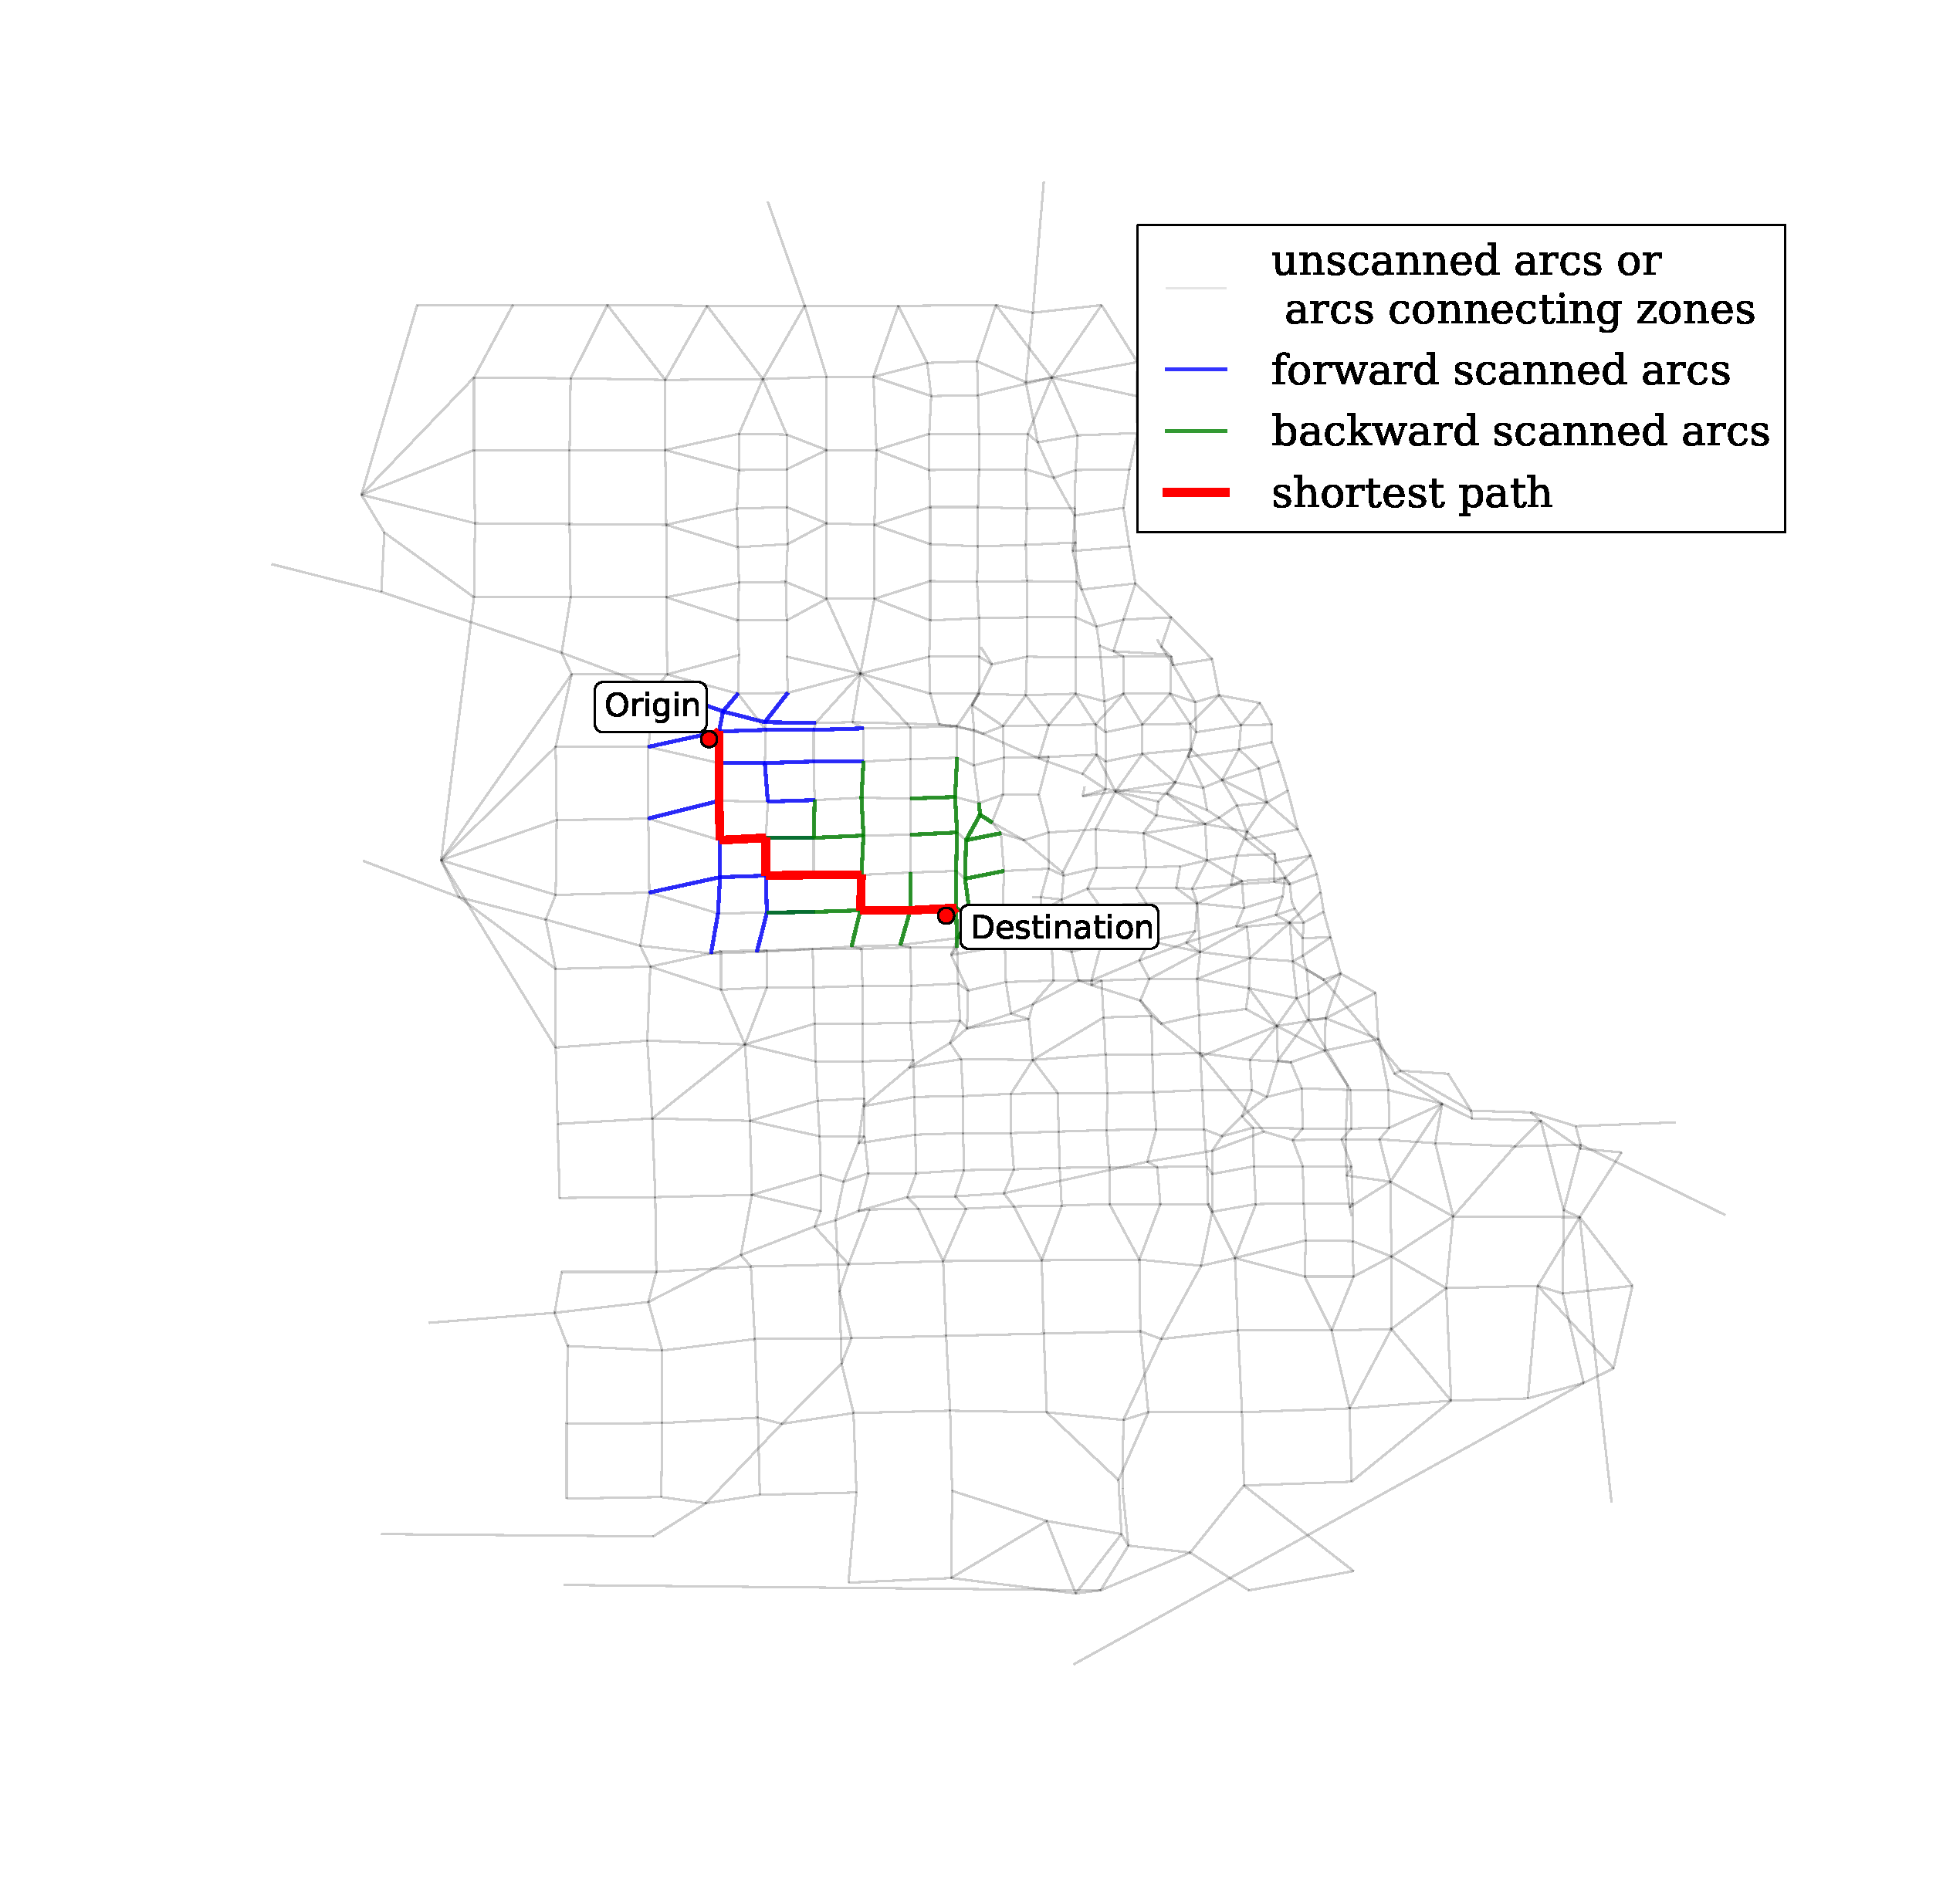
\includegraphics[width=\textwidth,trim=120px 120px 48px 0px,clip]{img/chicago_astar_bidirect2}
        \caption{Bidirectional A* Search}
        \label{fig:chicago_astar_bidirect2}
    \end{subfigure}
    \vspace{1em}
    \caption{Shortest path tree between two close nodes in the ChicagoSketch Network}
    \label{fig:short_sptree}
\end{figure}



All of these run times are slower than the STL version of the Heap.
Upon inspection,
it is found that the increase-key operation is used about between 5\% to 10\%
of the time,
\todo{not actual count yet}
which means the graphs are not dense enough for these Heap structures to outperform a
simple array based priority queue.
Comparing the Dijkstra and A* search algorithm's result,
we see an approximately 5 times improvement.
By looking at the shortest path tree generated
by the ChicagoSketch network,
there are only a few scanned nodes,
the path goes straight to the destination.
(TODO reference) says the closer the heuristic is to the actual distance,
the better/faster shortest path calculation,
by looking at the travel time function (Figure~\ref{fig:flowfunction}, we can see the slope
is really shallow near the start,
and by comparing the initial flow and final flow (TODO, data),
they are very close so the final flow is very close to the
initial flow,
which means the heuristic is a very good estimation,
which is our A* search is very fast.

%The problem with this strategy is that we have to know how many iterations the algorithm will take and choose an appropriate number that is less than that,
%this is because choosing a `bad' skipping number will result either unnecessary computations or have no effect on reducing the run time.
